\documentclass{beamer}
\usepackage[utf8]{inputenc}
\usepackage{graphicx}
\usepackage{hyperref}
\usepackage{amsmath}
\usepackage{booktabs}
\usepackage{float}
\usepackage{xcolor}
\usepackage{enumitem}
% Removed fontspec package which can cause issues with pdflatex
\usepackage{microtype}

% Professional orange color scheme
\definecolor{maincolor}{RGB}{232, 126, 4} % Primary orange
\definecolor{secondcolor}{RGB}{89, 49, 4} % Dark orange/brown
\definecolor{accentcolor}{RGB}{255, 165, 0} % Bright orange
\definecolor{highlightcolor}{RGB}{255, 215, 0} % Golden highlight

% Beamer theme settings
\usetheme{Madrid}
\usecolortheme{beaver}
\setbeamercolor{structure}{fg=maincolor}
\setbeamercolor{title}{fg=maincolor}
\setbeamercolor{frametitle}{fg=maincolor, bg=white}
\setbeamercolor{block title}{bg=maincolor!20, fg=secondcolor}
\setbeamercolor{block body}{bg=maincolor!10}
\setbeamercolor{itemize item}{fg=maincolor}
\setbeamercolor{itemize subitem}{fg=maincolor}
\setbeamertemplate{navigation symbols}{}
\setbeamertemplate{footline}[frame number]

% Title formatting with more space and cleaner design
\setbeamertemplate{frametitle}{
    \vspace*{0.5cm}
    \begin{beamercolorbox}[wd=\paperwidth,sep=0.5cm]{frametitle}
        \usebeamerfont{frametitle}\insertframetitle
    \end{beamercolorbox}
    \vspace*{0.1cm}
    \hrule height 1.5pt \textcolor{maincolor}{}
    \vspace*{0.3cm}
}

% Item formatting with better spacing
\setlist[itemize]{leftmargin=*,label=\textcolor{maincolor}{$\bullet$}, itemsep=0.8em}
\setbeamerfont{itemize/enumerate body}{size=\large}
\setbeamerfont{itemize/enumerate subbody}{size=\normalsize}

% Increase font size for better readability
\setbeamerfont{title}{size=\LARGE\bfseries}
\setbeamerfont{subtitle}{size=\large}
\setbeamerfont{frametitle}{size=\Large\bfseries}
\setbeamerfont{block title}{size=\large\bfseries}

\title{\textcolor{maincolor}{\LARGE PyTorch Capstone Project}}
\subtitle{\textcolor{secondcolor}{Cat Breed Classification System}}
\author{\textcolor{secondcolor}{Wiwat Pholsomboon}}
\date{\textcolor{secondcolor}{April 8, 2025}}

\begin{document}

\begin{frame}
    \titlepage
    % Commented out the problematic image
    % \begin{center}
    %     \includegraphics[width=0.2\textwidth]{cat_icon.png}
    % \end{center}
    \begin{center}
        \textcolor{secondcolor}{Deep Learning with Pytorch - INFO-6147-(01)-25W}
    \end{center}
\end{frame}

\begin{frame}{Introduction}
    \begin{itemize}
        \item Study on using PyTorch models to classify cat breeds
        \item Implementation of Grad-CAM for visual explanation
        \item Integration with ChatGPT-4o-mini for image identification
        \item Interactive quiz system to compare model accuracy with human performance
    \end{itemize}
\end{frame}

\begin{frame}{Dataset}
    \begin{itemize}
        \item \textbf{Source:} Kaggle 'Geno Cat Breed Image Collection'
        \item \textbf{Size:} 15 cat breeds with 375 photos each (5,625 total)
        \item \textbf{Preprocessing pipeline:}
        \begin{itemize}
            \item Resize to 256×256 pixels
            \item Random crop to 224×224 pixels
            \item Random horizontal flip for augmentation
            \item Random rotation for variety
            \item Conversion to PyTorch tensors
            \item Normalization using ImageNet statistics
        \end{itemize}
    \end{itemize}
\end{frame}

\begin{frame}{Model Architecture}
    \begin{columns}[T]
        \column{0.48\textwidth}
        \textbf{\textcolor{maincolor}{Custom CNN:}}
        \begin{itemize}
            \item 5 Convolutional layers
            \item 2 Fully connected layers
            \item Dropout for regularization
            \item ReLU activation functions
        \end{itemize}
        
        \column{0.48\textwidth}
        \textbf{\textcolor{maincolor}{Transfer Learning Models:}}
        \begin{itemize}
            \item ResNet18
            \item EfficientNetB2
            \item VGG16
            \item All pre-trained with ImageNet weights
        \end{itemize}
    \end{columns}
\end{frame}

\begin{frame}{Training Methodology}
    \begin{center}
        \textbf{\textcolor{maincolor}{Consistent hyperparameters across all models:}}
    \end{center}
    \vspace{0.5cm}
    \begin{columns}[T]
        \column{0.48\textwidth}
        \begin{itemize}
            \item Batch size: 128
            \item Learning rate: 0.001
            \item Momentum: 0.9
        \end{itemize}
        
        \column{0.48\textwidth}
        \begin{itemize}
            \item Epochs: 5
            \item Loss function: Cross Entropy
            \item Optimizer: SGD
        \end{itemize}
    \end{columns}
\end{frame}

\begin{frame}{Results and Evaluation}
    % Placeholder for image - uncomment when file is available
    \begin{center}
        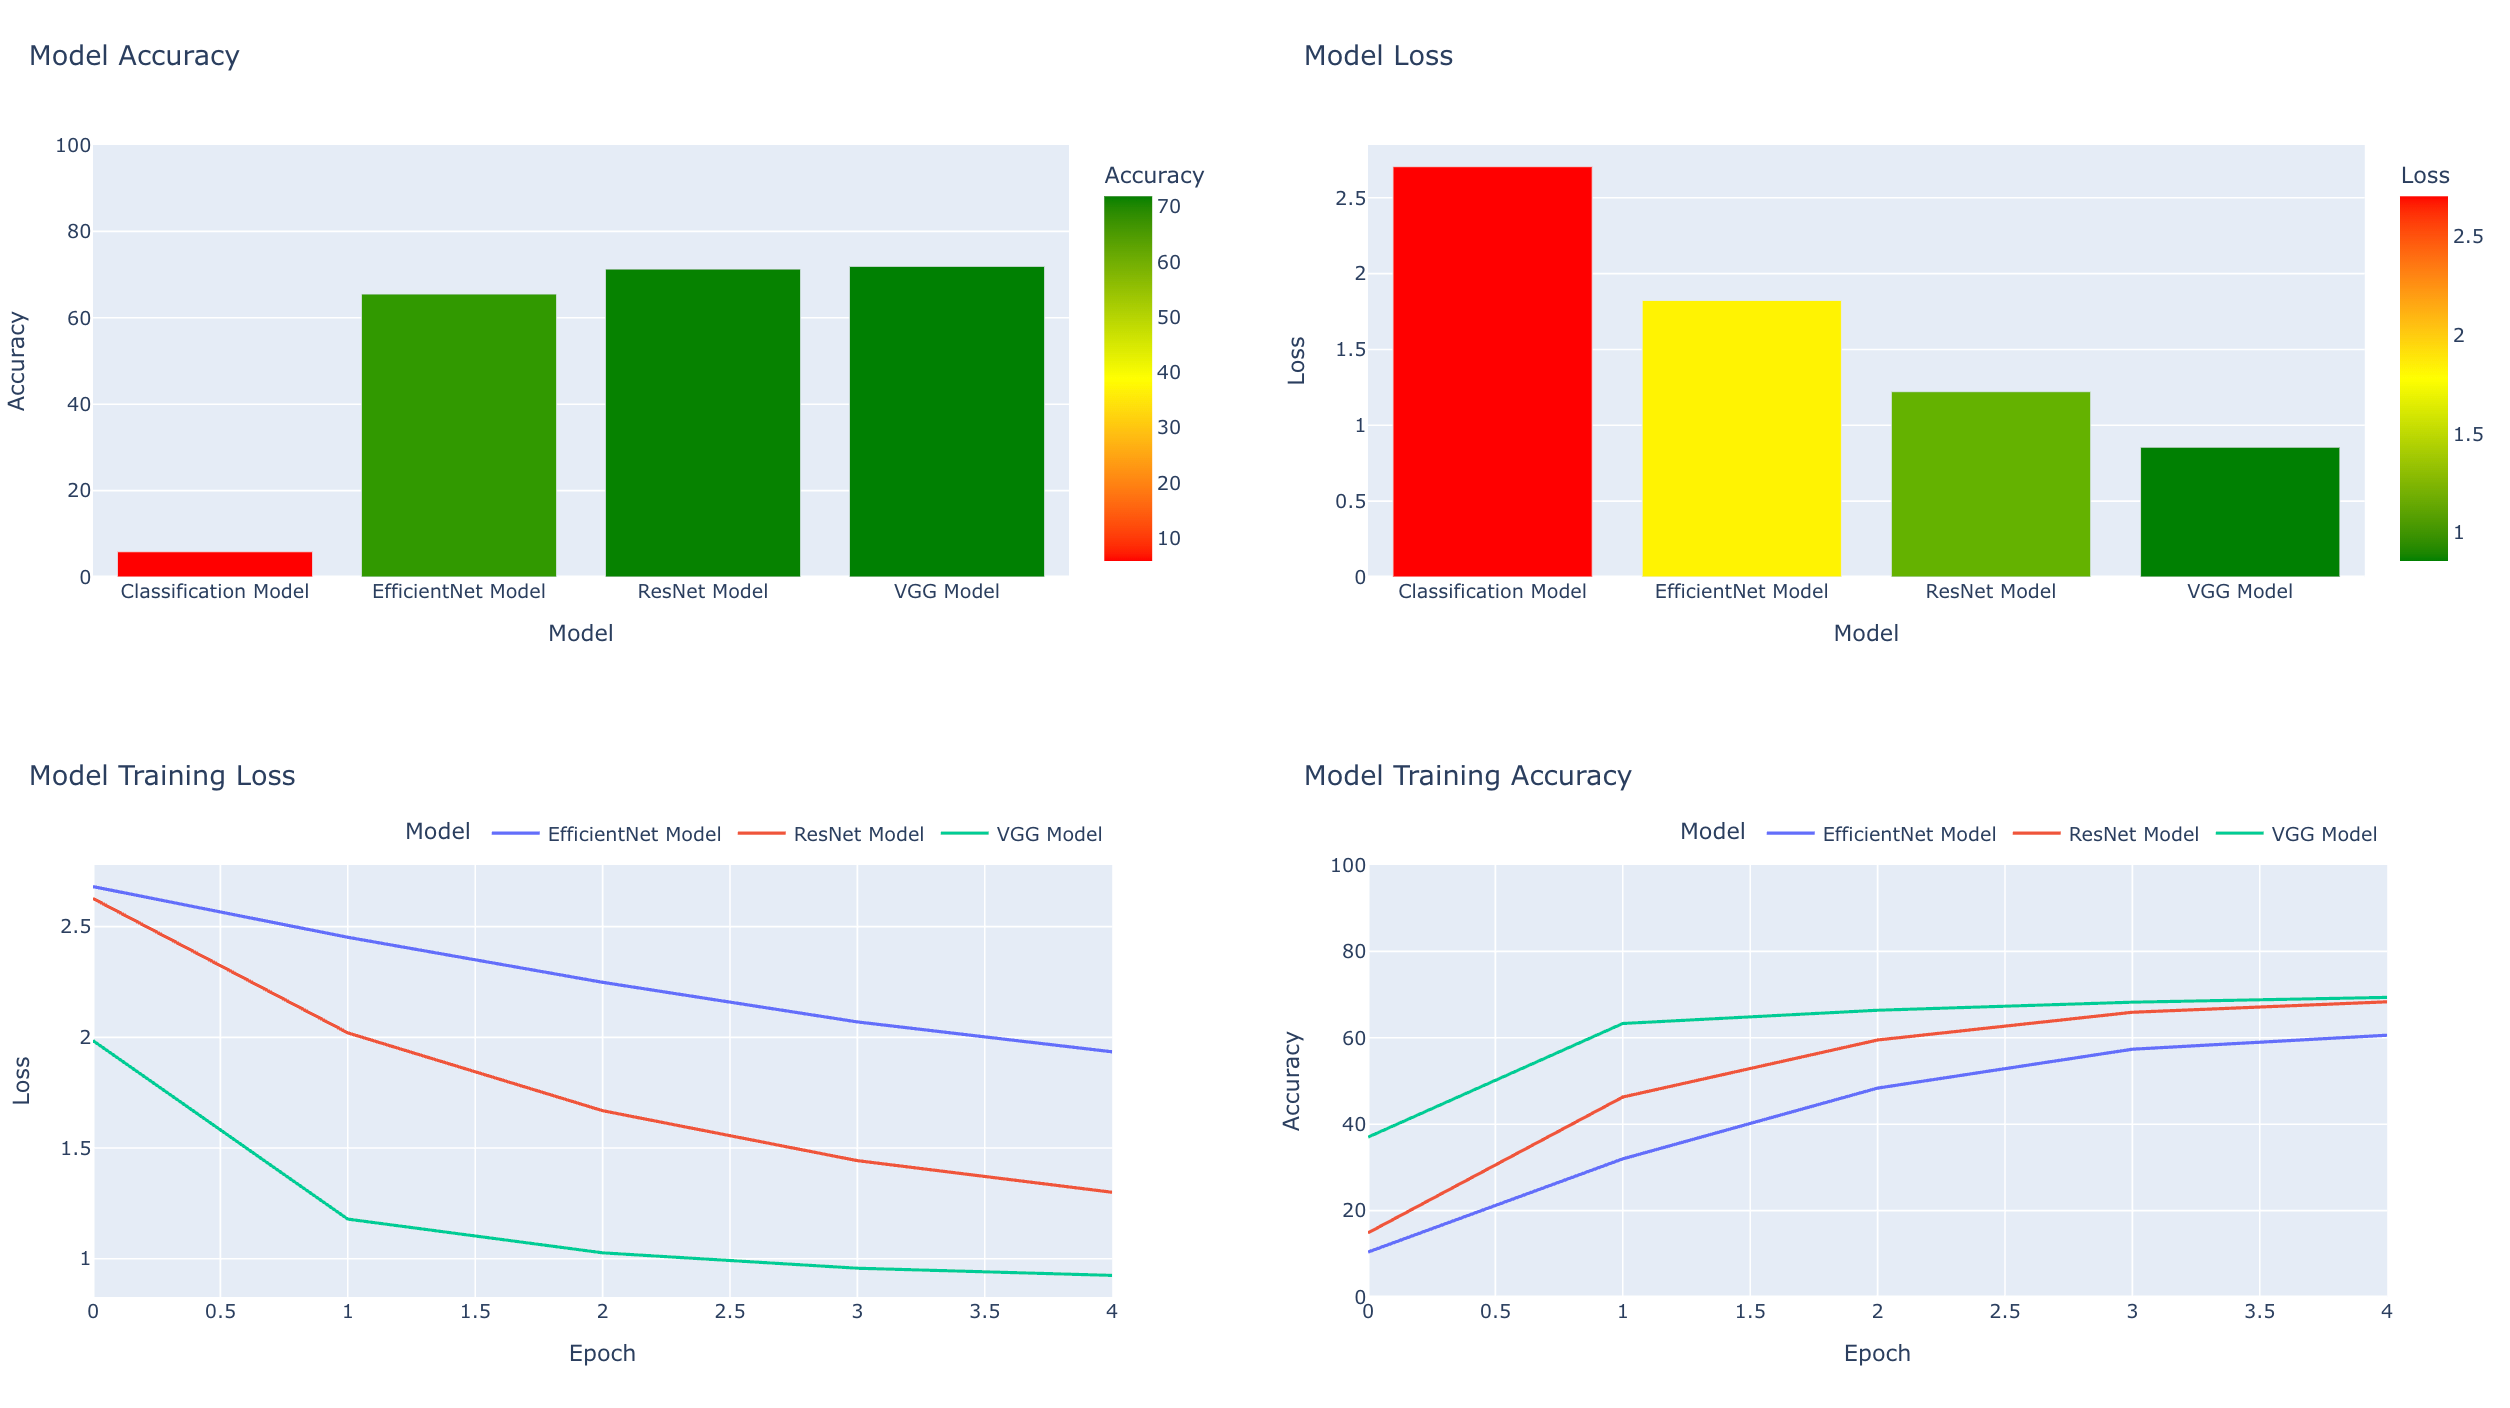
\includegraphics[width=0.65\textwidth]{models.png}
    \end{center} 
    \begin{itemize}
        \item Comparison of model accuracy and loss
        \item Interactive quiz implementation for human vs AI performance analysis
    \end{itemize}
\end{frame}

\begin{frame}{Visualization and Interpretability}
    \begin{columns}[T]
        \column{0.48\textwidth}
        % Placeholder for image - uncomment when file is available
        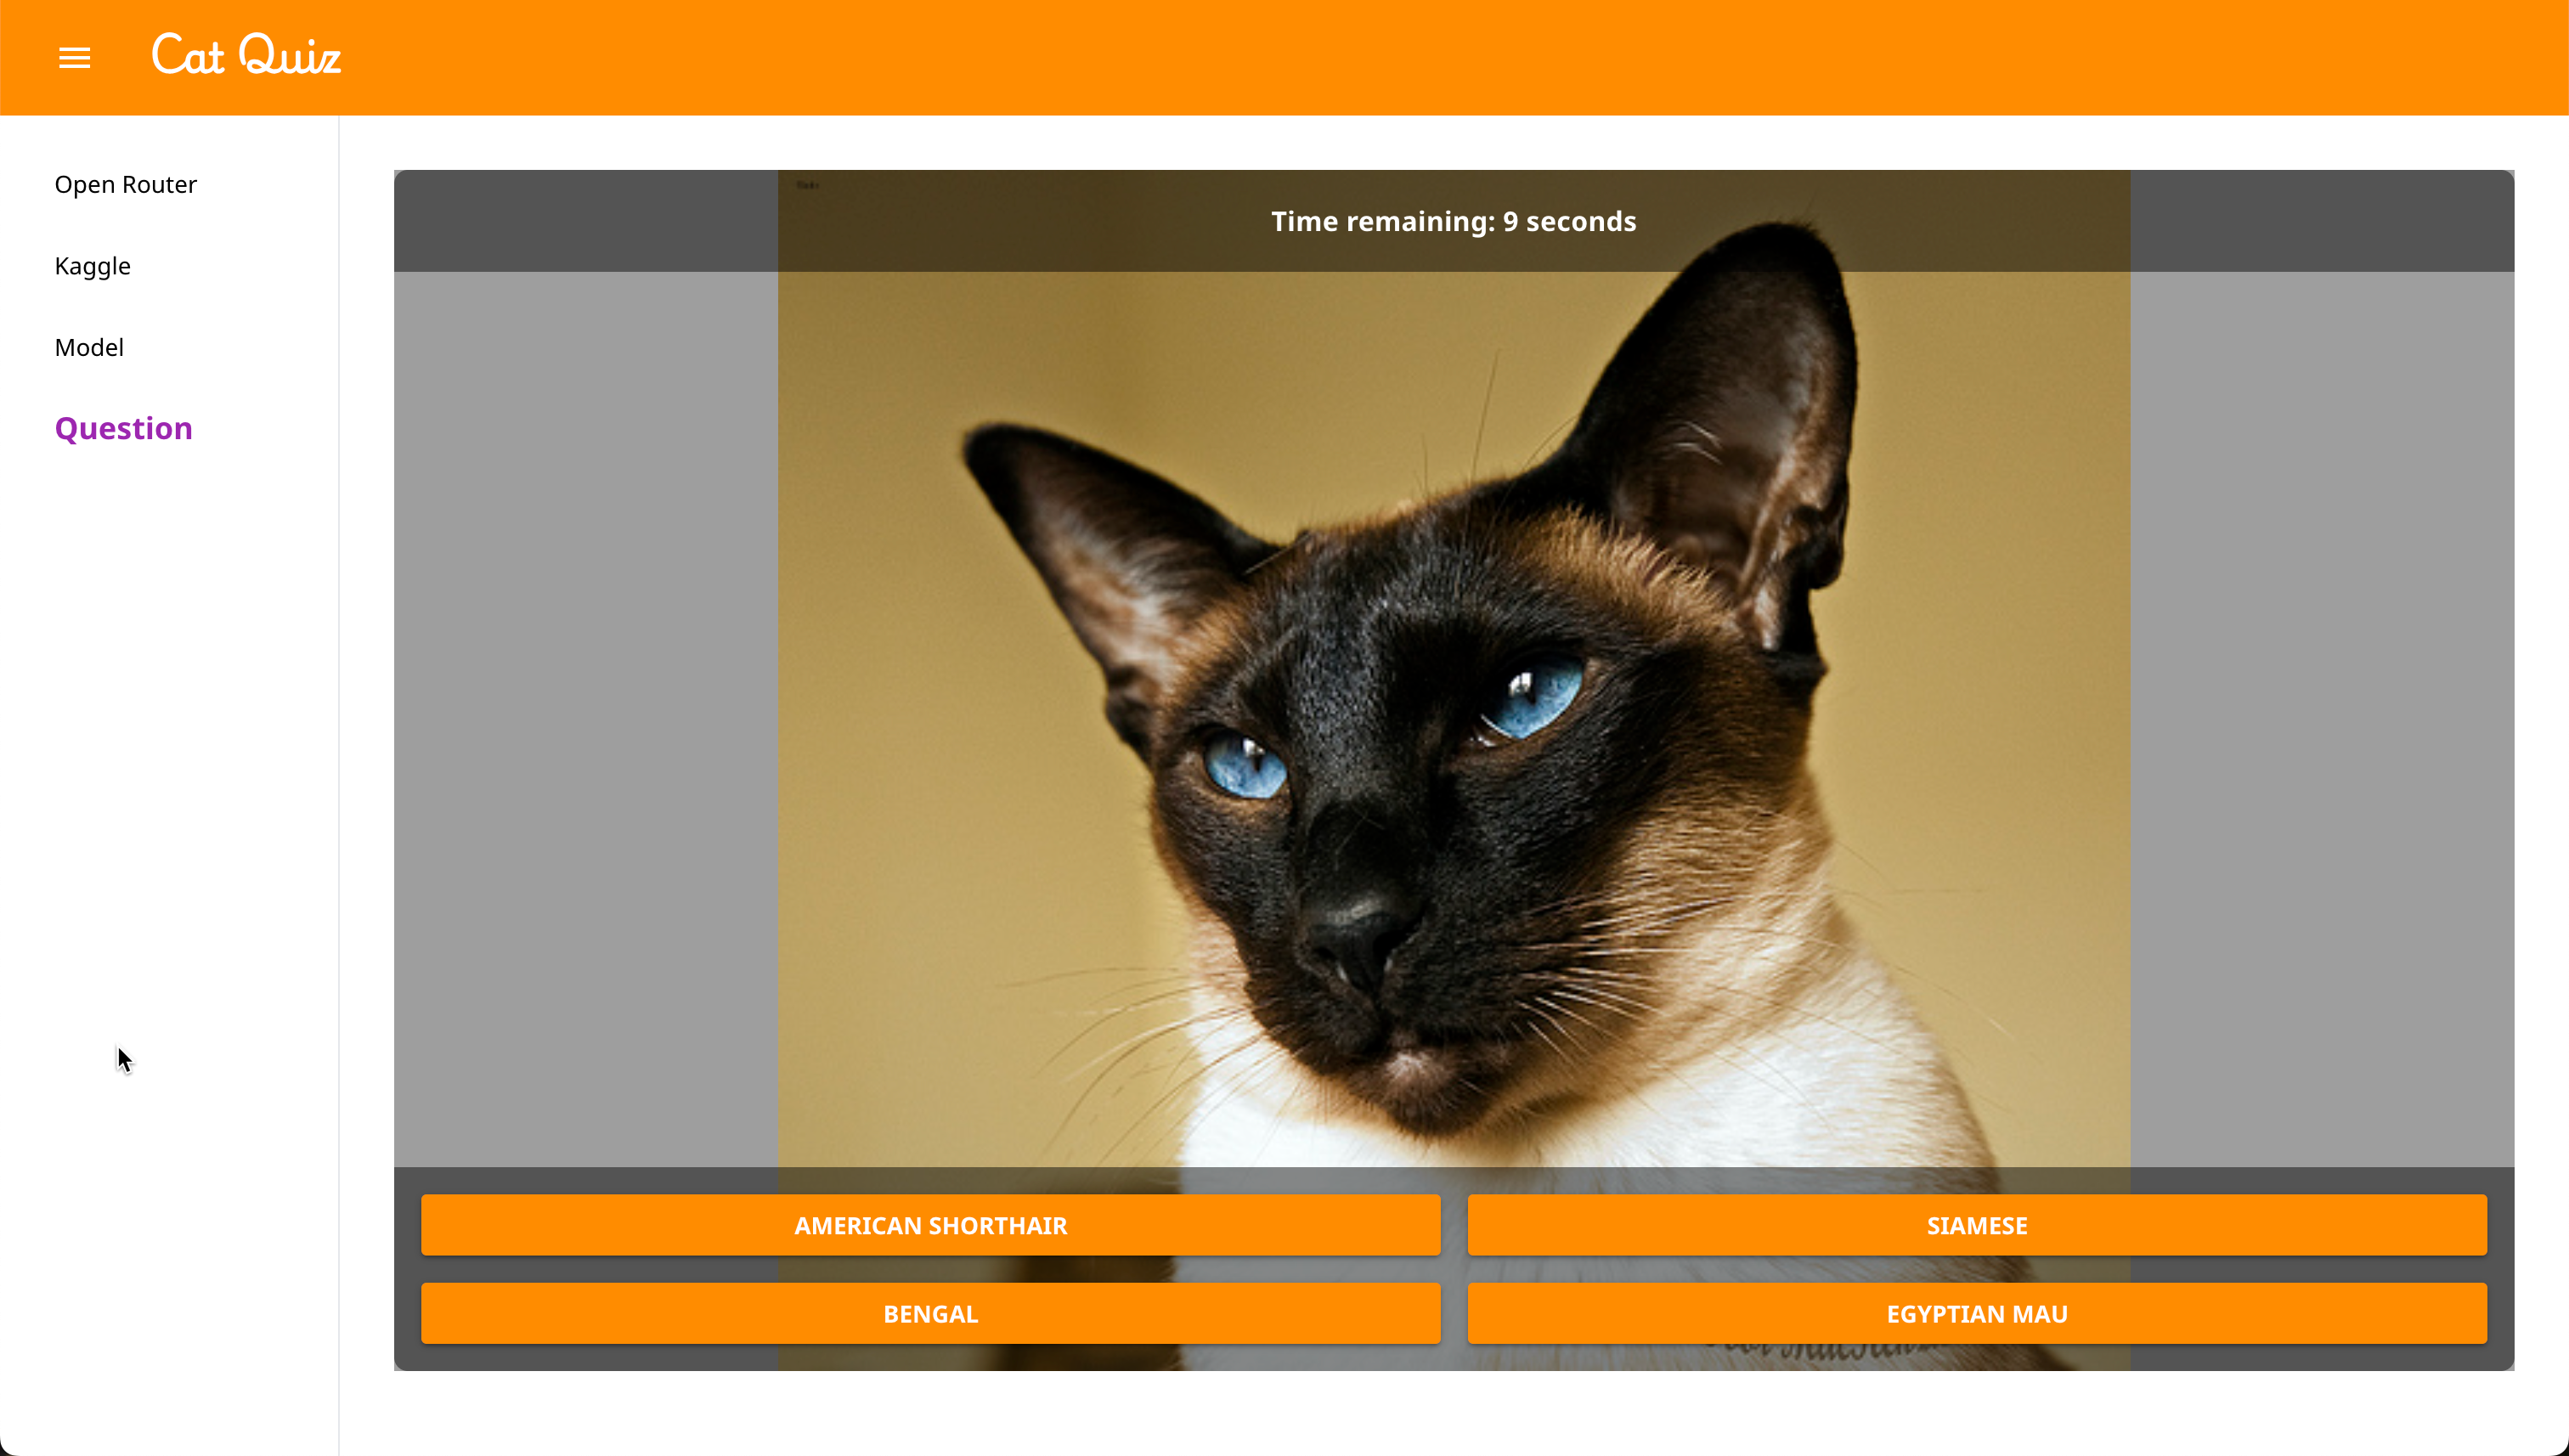
\includegraphics[width=\textwidth]{quiz.png}
        
        \column{0.48\textwidth}
        \begin{itemize}
            \item \textbf{Grad-CAM visualization} highlights regions of interest
            \item \textbf{ChatGPT-4o-mini} provides reasoning for predictions
            \item \textbf{Interactive interface} for user engagement
        \end{itemize}
    \end{columns}
\end{frame}

\begin{frame}{Evaluation Results}
    % Placeholder for image - uncomment when file is available

    \begin{itemize}
        \item Side-by-side comparison of accuracy:
        \begin{itemize}
            \item Human participants
            \item ChatGPT-4o-mini
            \item PyTorch models (CNN, ResNet, EfficientNet, VGG)
        \end{itemize}
    \end{itemize}    
    \begin{center}
        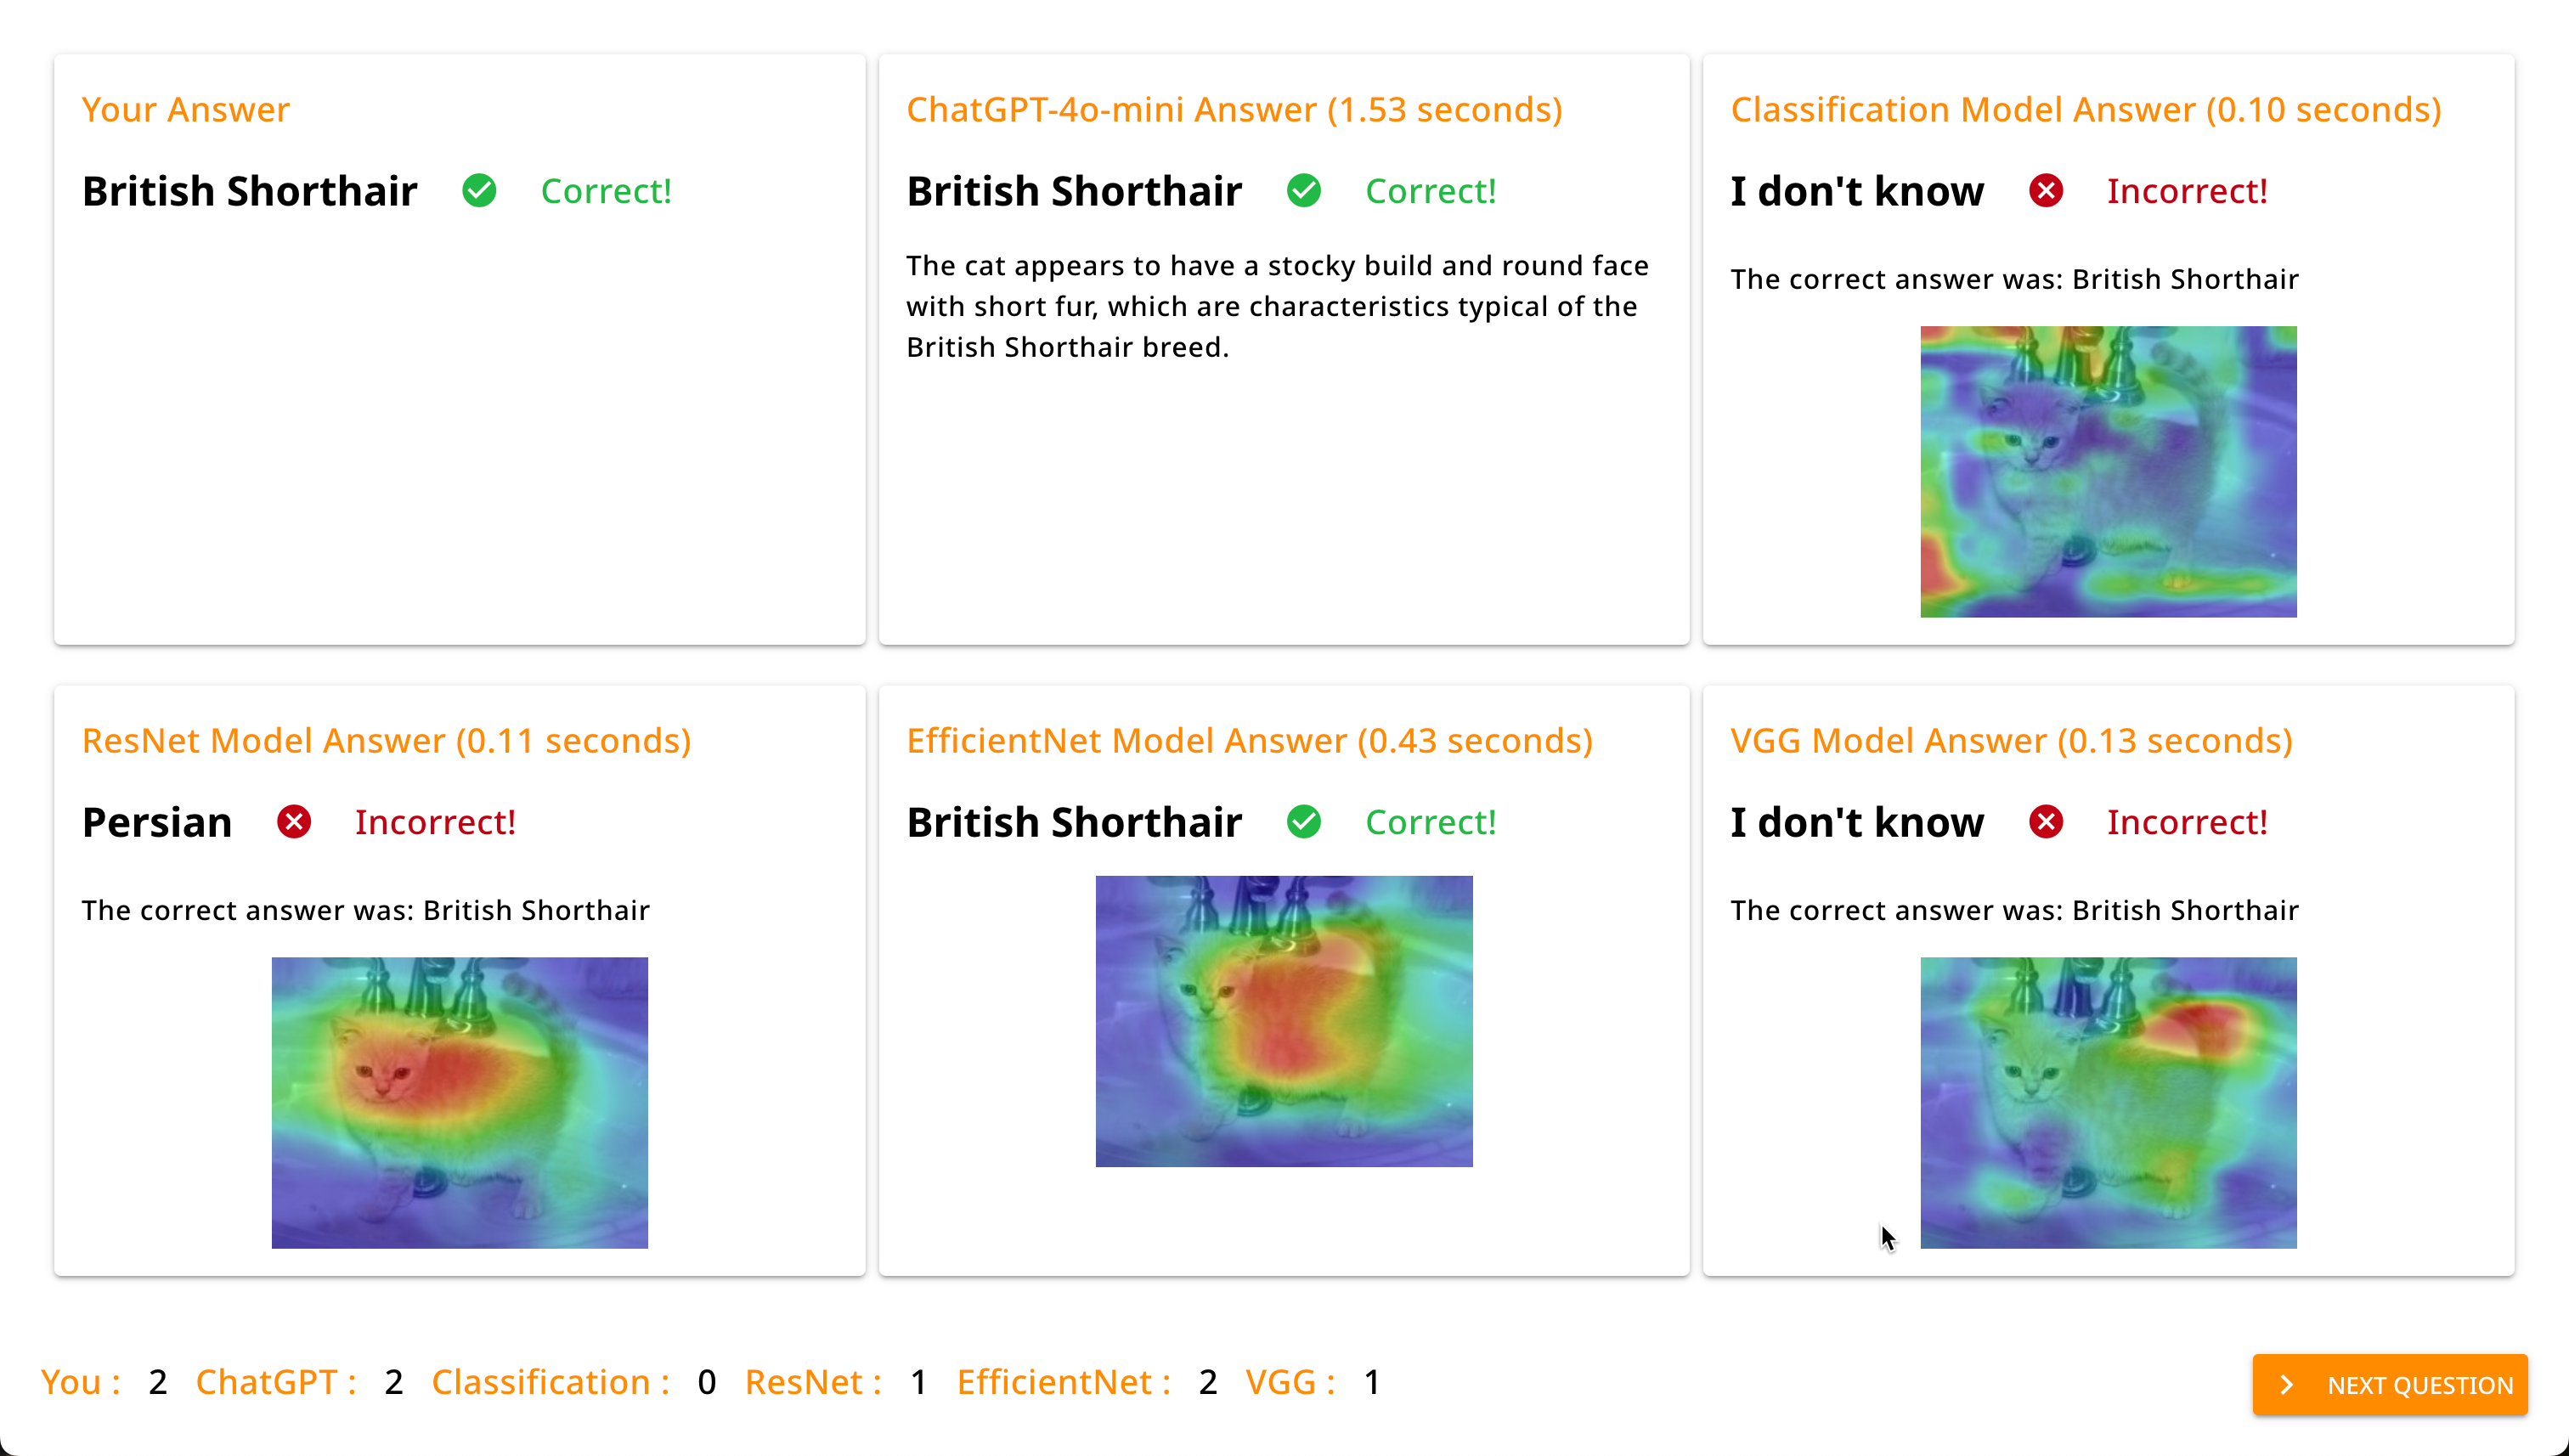
\includegraphics[width=0.55\textwidth]{evaluation.png}
    \end{center}
\end{frame}

\begin{frame}{Challenges and Solutions}
    \begin{columns}[T]
        \column{0.48\textwidth}
        \textbf{\textcolor{accentcolor}{Challenges:}}
        \begin{itemize}
            \item Different target layers for Grad-CAM across models
            \item Low accuracy with custom CNN model
        \end{itemize}
        
        \column{0.48\textwidth}
        \textbf{\textcolor{highlightcolor}{Solutions:}}
        \begin{itemize}
            \item Manual selection of appropriate CNN layers
            \item Transfer learning to leverage pre-trained weights
        \end{itemize}
    \end{columns}
\end{frame}

\begin{frame}{Future Improvements}
    \begin{block}{Potential Enhancements}
        \begin{itemize}
            \item User management system to track quiz performance over time
            \item Enhanced data augmentation techniques for better generalization
            \item Additional model architectures for comparison
            \item More comprehensive evaluation metrics beyond accuracy
            \item Fine-tuning of transfer learning models
        \end{itemize}
    \end{block}
\end{frame}

\begin{frame}{Conclusion}
    \begin{itemize}
        \item \textbf{ChatGPT-4o-mini} demonstrates superior accuracy due to advanced image understanding capabilities
        \item \textbf{Transfer learning models} perform moderately well with limited training
        \item \textbf{Custom CNN model} shows potential but requires more extensive training
        \item \textbf{Visualization tools} provide valuable insights into model decision-making
    \end{itemize}
    
    \vspace{0.5cm}
    \begin{center}
        \textbf{\textcolor{maincolor}{Thank you!}}
    \end{center}
\end{frame}

\end{document} 